\documentclass[10pt]{article}
\usepackage[T1]{fontenc}
\usepackage{ae,aecompl}
\usepackage[utf8x]{inputenc}

\usepackage{amsfonts}
\usepackage{amsmath}
\usepackage{amssymb}
\usepackage{amsthm}
\usepackage{booktabs}
%\usepackage{mathtools}
%\usepackage[cm]{fullpage}
\usepackage{graphicx}
\usepackage[numbers,sort&compress,square]{natbib}
\usepackage[pdftex,bookmarks=true,pdfstartview={FitH},pdfauthor={XXX},pdftitle={Approximate Query Processing with Confidence Bounds},pdfsubject={Approximate Query Processing}]{hyperref} % Must be included after natbib
\usepackage{subfig}
\usepackage{url}

% Temporary Packages
\usepackage{fullpage}
\usepackage[show]{notes-alt}
\usepackage{times}

%\newtheorem{proof}{Proof}
\newtheorem{corollary}{Corollary}
\newtheorem{conj}{Conjecture}
\newtheorem{claim}{Claim}
\newtheorem{fact}{Fact}
\newtheorem{lemma}{Lemma}
\newtheorem{theorem}{Theorem}

\theoremstyle{definition}
\newtheorem{definition}{Definition}

\newcommand{\Db}{{\cal D}}
\newcommand{\Sam}{{\cal S}}
\newcommand{\Tab}{{\cal T}}
\newcommand{\VC}{\mathsf{VC}}
\newcommand{\Out}{\mathsf{Out}}
\newcommand{\vc}{\mathsf{vc}}
\newcommand{\card}{\mathsf{c}}
\newcommand{\selectivity}{\sigma}
\newcommand{\domain}[1]{\mathsf{D}\left(#1\right)}
\newcommand{\values}[1]{\mathsf{V}\left(#1\right)}
\newcommand{\multivalues}[1]{\mathsf{M}\left(#1\right)}
\newcommand{\SELECT}{\mbox{\texttt{SELECT }}}
\newcommand{\FROM}{\mbox{\texttt{ FROM }}}
\newcommand{\WHERE}{\mbox{\texttt{ WHERE }}}
\newcommand{\AND}{\mbox{\texttt{ AND }}}
\newcommand{\GROUPBY}{\mbox{\texttt{ GROUP BY }}}

\DeclareMathOperator{\op}{op}
\DeclareMathOperator{\bool}{bool}
\DeclareMathOperator{\eqop}{eqop}

\begin{document}
\title{Approximate Query Processing with Confidence Bounds}
\author{}
\maketitle

\begin{abstract}
  We present a new method to compute high quality approximations of aggregate
  database queries. Our method executes the queries on a fixed static sample of the original
  database, created off-line. It does not require any information about the
  underlying data distribution. The sample size does not depend on the size of
  the dataset but only on the complexity of the class of queries to be run,
  expressed through the VC-Dimension of the class. An upper bound to this
  quantity can be easily computed from the SQL expression of the queries. The
  values computed by running the queries on the sample are, with high
  probability, good approximations to the real values. To quantify the accuracy
  of the estimated value, we develop a method  to compute confidence intervals
  around the estimation. This method is based on a convex
  optimization problem, which can be efficiently solved using known techniques.
  With high probability the confidence intervals contain the real values, for
  all queries. To our knowledge this is the first work that can achieve this
  guarantee for all queries in a given class simultaneously. We performed an
  extensive experimental evalution of our methods, showing that they achieve
  high accuracy and great speed-up compared to running the queries on the
  original dataset.
\end{abstract}


\section{Introduction}\label{sec:intro}
\todo{Write.

Ideas:
\begin{itemize}
  \item Aggregate queries gives you an intuition, a condensed piece of
    information, a rough picture of the data. The collection of statistics has
    somewhat an exploratory flavour.
  \item Computing them exactly is not worth it at takes a lot of time due to the
    desire to squeeze each possible bit of information from the database.
  \item Given the goal, it is actually ok to settle for approximate answers.
    These still give enough information about the data, and they 
  \item Online aggregation bad (slow)
  \item Guarantees are important. Not easy to achieve guarantees over all the
    queries. Need to use more powerful statistical techniques.
\end{itemize}
}

\paragraph{Our Contributions.} In this work we introduce a new method for
computing \emph{high-quality approximate answers to aggregate queries}. We run
queries on a \emph{fixed static sample} of the dataset created off-line. The
method does not make any assumption on the distribution of the data in the
database, i.e., it is \emph{distribution-free}. It does not requires any
knowledge of the workload except for the
\emph{maximum complexity} of the queries that the user is interested in running. Our
definition of complexity depends on the maximum number $b$ of conditions in
the selection predicate, the maximum number $m$ of columns the maximum number of
joins $u$. Starting from this information, our method derives a sample size
such that a random sample of the database of that size can be used to compute good
approximations of the values of all the queries with the specified complexity by
running the queries on the sample. The sample fits in main memory and is computed only once off-line and only
needs to be updated after major changes in the original database. This results
in a huge speedup in the execution of the queries. Given two user-specified
parameters $\varepsilon$ and $\delta$ which control the
accuracy and the confidence of the approximate answers, the sample size is
$O(\varepsilon^{-2}(\mathsf{poly}(b,m,u)+\log(1/\delta)))$ and it does not depend
on the size of the original database, but only on the maximum query complexity
and on $\varepsilon$ and $\delta$. Deriving such a sample size is possible thanks to an
application of VC-dimension theory to database queries. In order to be more
informative about the quality of the approximate answers, we also developed a
method based compute \emph{deterministic confidence intervals} for the answers.
The confidence intervals can be computed efficiently, as the method requires the
solution of a \emph{convex optimization problem}. We can guaranteed that, with
probability at least $1-\delta$, the computed interval will contain the true
value of the aggregate query for all queries \emph{simultaneously}. We conducted
an extensive experimental evaluation of the accuracy of our estimations and
confidence intervals and of the speedup achieved by our method, showing that it
is very accurate and fast.
\todo{We are missing stuff like ``we are the first to do this and that''. We are
also not saying anything about group-by queries.}

\paragraph{Outline.} We introduced the basic definitions, concepts and tools in
Sect.~\ref{sec:prelims}. Our methods for computing good approximations of
aggregate queries and deterministic confidence intervals is presented in
Sect.~\ref{sec:aggreg}. We conducted an extensive experimental evaluation of our
approach and report the results in Sect.~\ref{sec:exper}.
Sect.~\ref{sec:prevwork} contains a review of the relevant previous work.  We
wrap up with conclusions and future work in Sect.~\ref{sec:concl}.
\note{At the moment we are following the ``database/system'' style of putting
previous work at the end. We may change that in the future.}


\section{Preliminaries}\label{sec:prelims}
In this section, we introduce the necessary terminology, concepts, and tools
that we will use to develop our results in the following sections.

\subsection{Databases and Queries}\label{sec:dbqueries}
We outline here some basic definitions about databases, queries, and
selectivity. We refer the reader to complete textbooks for additional
information~\citep{GarciaMolinaUW02}.
We consider a \emph{database} $\Db$ of $k$ tables $\Tab_1,\dotsc,\Tab_k$. 
A \emph{table} $\Tab$ is a two-dimensional representation of data. It
contains a number of rows or \emph{tuples}, and may (and typically does) have multiple
\emph{columns}. We denote a column $C$ of a table $\Tab$ as $\Tab.C$ and, for a
tuple $t\in\Tab$, the value of $t$ in the column $C$ as $t.C$. We denote the
domain of the values that can appear in a column $\Tab.C$ as $\domain{\Tab.C}$.
Each tuple $t$ is then an element from the Cartesian product of the domains of
the columns of $\Tab$, $t\in \domain{\Tab.C_1}\times\dotsb\times
\domain{\Tab.C_m}$. Figure~\ref{tab:example} shows two examples of database
tables, \emph{Customers} and \emph{CarColors}. 

\begin{figure}[htb]
  \begin{subtable}[b]{0.6\textwidth}
    \centering
    \begin{tabular}{c|c|c|c|c}
      %\toprule
      \multicolumn{5}{c}{\emph{Customers}} \\
      \midrule
      \emph{Name} & \emph{Age} & \emph{Street} & \emph{ZipCode} & \emph{CarBrand} \\
      \midrule
      \texttt{John Doe} & \texttt{20} & \texttt{Pratt Av.} & \texttt{02906} & \texttt{BMW} \\
      \texttt{Jim Clark} &  \texttt{30} &\texttt{Morris Rd.} & \texttt{02906} & \texttt{Lotus} \\
      \texttt{Greta Garbo} & \texttt{60} & \texttt{Pratt Av.} & \texttt{05902} & \texttt{Rolls-Royce} \\
      \bottomrule
    \end{tabular}
    \caption{A table with four columns}
  \end{subtable}
  \hfill
  \begin{subtable}[b]{0.3\textwidth}
    \centering
    \begin{tabular}{c|c}
      \multicolumn{2}{c}{\emph{CarColors}} \\
      \midrule
      \emph{Name} & \emph{Color} \\
      \midrule
      \texttt{John Doe} & \texttt{Black} \\
      \texttt{Jane Doe} & \texttt{Red} \\
      \texttt{Greta Garbo} & \texttt{Red}\\ 
      \bottomrule
    \end{tabular}
    \caption{A table with two columns}
  \end{subtable}
  \caption{Example of two database tables.}
  \label{tab:example}
\end{figure}

A \emph{query} $q$ is a function that takes as input one or more tables and
returns a set of elements the Cartesian product of the input tables. This set
depends on the database $\Db$ which the input tables to $q$ belong to, and we
denote with $\Out_\Db(q)$ and we call it the output of $q$ on $\Db$. The
\emph{cardinality} $\card_\Db(q)$ of $q$ on $\Db$ is the size
$|\Out_\Db(q)|$. The \emph{selectivity} $\selectivity_\Db(q)$ of $q$ on $\Db$ is
the ratio between $\card_\Db(q)$ and the \emph{product} of the sizes of the
input tables of $q$.  Clearly, $0\le\selectivity_\Db(q)\le 1$.

There are many different types of queries. We now introduce the ones we are interested
in for our purposes.
\begin{definition}\label{def:selectquery}
  Given a table $\Tab$ with columns $\Tab.C_1,\dotsc,\Tab.C_\ell$, a
  \emph{selection query} $q$ on $\Tab$ is a function which returns a subset
  $S$ of the tuples of $\Tab$ such that a tuple $t$ of $\Tab$ belongs to $S$ if
  and only if the values in $t$ satisfy a condition $\mathcal{C}$
  (the \emph{selection predicate}) expressed by $q$. In full
  generality, $\mathcal{C}$ is the Boolean combination of clauses of the form
  ``$\Tab.C_i \op a_i$'', where $\Tab.C_i$ is a column of $\Tab$, ``$\op$'' is one
  of $\{<,>,\ge,\le,=,\neq\}$ and $a_i$ is an element of the domain of
  $\Tab.C_i$.
\end{definition}

As an example, the selection query 
\[
\SELECT * \FROM \text{\emph{Customers}} \WHERE \text{\emph{Customers.ZipCode}} = 02906;
\]
would return the first and second row of Table~\ref{tab:example}.

\note{Maybe the following should go on top, rephrased.}
We assume that, for each column $\Tab_C$ of each table $\Tab$, the domain
$\domain{\Tab.C_i}$ is such that it is possible to build a total order relations
on it. This assumptions does not exclude categorical domains from our
discussion, because the only meaningful values for ``$\op$'' for such domains
are ``$=$'' and ``$\neq$'', so we can just assume an arbitrarily but fixed order
for the categories in the domain.

\begin{definition}\label{def:joinquery}
  Given two tables $\Tab_1$ and $\Tab_2$, a $\emph{join query}$ $q$ on a common
  column $C$ (i.e., a column present both in $\Tab_1$ and $\Tab_2$) is a
  function which returns a subset of the Cartesian product of the tuples in
  $\Tab_1$ and $\Tab_2$. The returned subset is defined as the set $ \{(t_1,t_2)
  ~:~ t_1\in\Tab_1, t_2\in\Tab_2, \text{ s.t. } t_1.C \op t_2.C \}$ where
  ``$\op$'' is one of $\{<,>,\ge,\le,=,\neq\}$.
%  A join query can be expressed in SQL as
%  \[
%    \SELECT * \FROM \Tab_1,\Tab_2 \WHERE \Tab_1.C \op \Tab_2.C;
%    \]
  The condition $\Tab_1.C \op \Tab_2.C$ is known as the \emph{join predicate}
  $\mathcal{C}$.
\end{definition}
An example of a join query is the following:
\[
\SELECT * \FROM \text{\emph{Customers}, \emph{CarColors}} \WHERE \text{ 
\emph{Customers.Name}} = \text{\emph{CarColors.Name}};
\]
This query would return the following tuples:
\begin{align*}
  &(\text{John Doe}, 21, \text{Pratt Av.}, \text{02906}, \text{BMW}, \text{Black}), \\
  &(\text{Greta Garbo}, 60, \text{Pitman St.}, \text{05902}, \text{Rolls-Royce}, \text{Red})
\end{align*}
The column \emph{Name} is reported only once for clarity.

Our definition of a join query is basically equivalent to that of a
\emph{theta-join}~\citep[Sect.5.2.7]{GarciaMolinaUW02}, with the limitation that
the join condition $\mathcal{C}$ can only contain a single clause, i.e., a single
condition on the relationship of the values in the shared column $C$ and only
involve the operators $\{<,>,\ge,\le,=,\neq\}$ (with their meaning on
$\domain{C}$). The pairs of tuples composing the output of the join in our
definition have a one-to-one correspondence with the tuples in the output of the
corresponding theta-join.

\begin{definition}\label{def:general query}
  Given a set of $\ell$ tables $\Tab_1,\dotsc,\Tab_\ell$, a \emph{combination of
  select and join queries} is a function that returns a subset of the Cartesian
  product of the tuples in the sets $S_1,\dotsc,S_\ell$, where $S_i$ is the
  output of a selection query on $\Tab_i$. The returned set is defined by the
  selection queries and by a set of join queries on $S_1,\dotsc,S_\ell$.
 % A combination of select and join operations can be expressed in SQL as
 % \[
 %   \SELECT * \FROM \Tab_1,\dotsc,\Tab_\ell \WHERE \mathcal{C};
 %   \].
 The condition $\mathcal{C}$ is the \emph{select/join predicate}, a Boolean combination
  of selection and join predicates.
\end{definition}

As an example, the query 
\begin{align*}
\SELECT &* \FROM \text{\emph{Customers},
\emph{CarColors}} \WHERE 
\text{\emph{Customers.Name}} = \text{\emph{CarColors.Name}} \\
& \AND \text{\emph{Customers.ZipCode}}=02906 \AND
\text{\emph{CarColors.Color}}=\text{\emph{Red}};
\end{align*}
combines select and joins operations. It returns no tuple (empty answer), as
there is no individual reported in both tables with zipcode $02906$ and a red
car.

When not further specified, we use the term ``query'' to denote a combination of
select and join queries.

\begin{definition}\label{def:groupbyquery}
  Let $\Db$ be a set of tables $\Db=\{\Tab_1,\dotsc,\Tab_\ell\}$, and
  $\mathcal{G}=\{G_1,\dotsc,G_k\}$ be a subset of the columns in the tables of $\Db$. For
  each $G_i$, let $\values{G_i}$ be the set of values in the column
  $G_i$ of the tuples in the tables $G_i$ belongs to (it may be $\values{G_i}\subset
  \domain{G_i}$). A \emph{group-by query} $q$ is a pair $(q^*,\mathcal{G})$ where $q^*$ is a query
  on $\Db$ and $\mathcal{G}$ is defined as above.  The output of $q$ is a
  \emph{partition} $\mathcal{P}$ of the output of $q^*$ such that there is a
  class $S_v\in\mathcal{P}$ for each element $v$ of the Cartesian product
  $\values{\mathcal{G}}=\values{G_1}\times \values{G_2}\times\dotsb\times
  \values{G_k}$. Each set $S_v$ contains the tuples from the output of $q^*$
  with values corresponding to $v$ on the columns $G_1,\dotsc,G_k$.

  A group-by query $(q^*,\mathcal{G})$ can be expressed in SQL as
  \[
  \SELECT * \FROM \Tab \WHERE \mathcal{C} \GROUPBY \mathcal{G};
   \]
  where $\mathcal{C}$ is the selection/join predicate of $q^*$.
\end{definition}
For example, the group-by query
\[
\SELECT * \FROM \text{\emph{Customers}}  \WHERE \text{\emph{Customers.Street}} =
\text{"Pratt Av."} \GROUPBY \text{\emph{Customers.ZipCode}}
\]
would return two sets, one for the value ``02906'' in \emph{Customers.ZipCode},
containing the first tuple of the \emph{Customers}
table, and one for the value ``05902'' containing the third tuple.

\begin{fact}\label{fact:groupbyequiv}
  Let $q=(q^*,\mathcal{G})$ be a group-by query as in Def.~\ref{def:groupbyquery}. 
  We can see the output of $q$ as the collection of the outputs of the queries
  in the set $\mathsf{GQ}(q)$ where $q_g\in \mathsf{GQ}(q)$ is a (non group-by)
  query such that $g=(g_1,\dotsc,g_k)\in \values{\mathcal{G}}$ and the
  selection/join predicate of $q_g$ is the selection/join predicate of $q$,
  denoted as $\mathcal{C}$, \texttt{AND}'ed with conditions involving the
  components of $g$:
  \begin{equation}\label{eq:groupbyequiv}
    \mathcal{C} \AND G_1=g_1 \AND \dotsb \AND G_k=g_k.
  \end{equation}
\end{fact}

\begin{definition}\label{def:aggregquery}
  Let $\Db=\{\Tab_1,\dotsc,\Tab_\ell\}$ be a set of tables, and let $\Tab\in \Db$,
  with a column $\Tab.C$. Let $\multivalues{\Tab.C}$ be the \emph{multiset} of
  values taken by tuples in $\Tab$ on the column $\Tab.C$. An \emph{aggregate
  query} $q$ is a pair $(q^*,f)$, where $q^*$ is a (potentially group-by) query
  on $\Db$, and $f$ is a function that maps subsets of $\multivalues{\Tab.C}$ to members
  of $\mathbb{R}$. The output of $q$ is the value taken by the function $f$ when
  applied to the subset of $\multivalues{\Tab.C}$ in the tuples in the output of $q^*$. If
  $q^*$ is a group-by query, $f$ is computed for every group and the output of
  $q$ is a set of values.  
\end{definition}
Typical examples for the function $f$ include sum (SQL operator \texttt{SUM}),
average (\texttt{AVG}), variance (\texttt{VAR}), standard
deviation (\texttt{STDEVP} \inote{There's STDEV and STDEVP. It's the usual $1/n$
vs $1/(n-1)$. Similar for VAR and VARP. Should take care of this.}), and median
and quantile computation \iquestion{Are there standard SQL expressions for these?}.
These are typically integrated in the query processing engine of commercial
database management systems. An example of an aggregate query is the following:
\[
\SELECT \text{\texttt{AVG}}(\text{\emph{Customers.Age}}) \FROM
\text{\emph{Customers}} \WHERE \text{\emph{Customers.ZipCode}} = 02906;
\]
The output of this query would be ``25'', the average between the values in the
\emph{Age} column in the first two tuples of the \emph{Customers} table.

\begin{fact}\label{fact:aggregquery}
  Let $f$ be a function as in Def.~\ref{def:aggregquery}, and let $A$ be a 
  subset of $\multivalues{\Tab.C}$. We can see $A$ as a collection of pairs
  $(v,c_v)$,
  where $v\in \domain{\Tab.C}$ and $c_v$ is a non-negative integer representing the number of
  times $v$ appears in $A$. So, $f$ can be seen as a function from
  $\mathcal{P}(\domain{\Tab.C}\times\mathbb{N}_0)$ to $\mathbb{R}$.
\end{fact}
For example, if we consider $f$ to be the average function, it is easy to see
that
\[
f(S)=\frac{1}{\sum_{(v,c_v)\in S} c_v}\sum_{(v,c_v)\in S}(vc_v), \forall
S\in\mathcal{P}(\domain{\Tab.C}\times\mathbb{N}_0)\enspace.\]

\subsection{VC-Dimension}\label{sec:prelvcdim}
The Vapnik-Chernovenkis (VC) Dimension of a space of points is a measure of the
complexity or expressiveness of a family of indicator functions (or equivalently
a family of subsets) defined on that space~\cite{VapnikC71}. A finite bound on
the VC-dimension of a structure implies a bound on the number of random samples
required for approximately learning that structure. We outline here some basic
definitions and results and refer the reader to the works
of~\citet[Sect.~14.4]{AlonS08},~\citet{MohriRT12} and~\citet{Vapnik99} for more details
on VC-dimension. %See Sect.~\ref{sec:prevwork} for applications of VC-dimension in computer science.

%VC-dimension is defined on {\em range spaces}:
%
%\begin{definition}\label{defn:rangespace}
We define a {\em range space} as a pair $(X,R)$ where $X$ is a (finite or infinite) set
 and $R$ is a (finite or infinite) family of subsets of $X$. The members of $X$
 are called {\em points} and those of $R$ are called {\em ranges}.
 %\end{definition}
%To define the VC-dimension of a range space we consider the projection of the
%ranges into a set of points:
%\begin{definition}\label{defn:proj}
%Let $(X,R)$ be a range space and $A\subset X$.
Given $A\subset X$, The {\em projection} of $R$ on
$A$ is defined as $P_R(A)=\{r\cap A ~:~ r\in R\}$.
%\end{definition}
%The VC-dimension is defined with respect to \emph{shattered} sets:
%
%\begin{definition}\label{defn:shatter}
%Let $(X,R)$ be a range space and $A\subset X$.
If $P_R(A)=2^A$, then $A$ is said to be {\em shattered by $R$}.
%\end{definition} 
The VC-dimension of a range space is the cardinality of the largest set
shattered by the space:
\begin{definition}\label{defn:VCdim}
  Let $S=(X,R)$ be a range space. The {\em Vapnik-Chervonenkis} dimension (or
  {\em VC-dimension}) of $S$, denoted as $\VC(S)$ is the maximum cardinality of
  a shattered subset of $X$. If there are arbitrary large shattered subsets,
  then $\VC(S)=\infty$.
\end{definition}

Note that a range space $(X,R)$ with an arbitrary large set of points $X$ and
an arbitrary large family of ranges $R$ can have a bounded VC-dimension. A simple
example is the family of intervals in $[0,1]$ (i.e., $X$ is all the points in
$[0,1]$ and $R$ all the intervals $[a,b]$, such that $0\leq a\leq b\leq 1$). Let
$A=\{x,y,z\}$ be the set of three points $0<x<y<z<1$. No interval in $R$ can
define the subset $\{x,z\}$ so the VC-dimension of this range space is less than
3~\cite[Lemma 10.3.1]{Matousek02}. Another example is shown in
Fig.~\ref{fig:rectangles}.
\begin{figure}[ht]
  \centering
  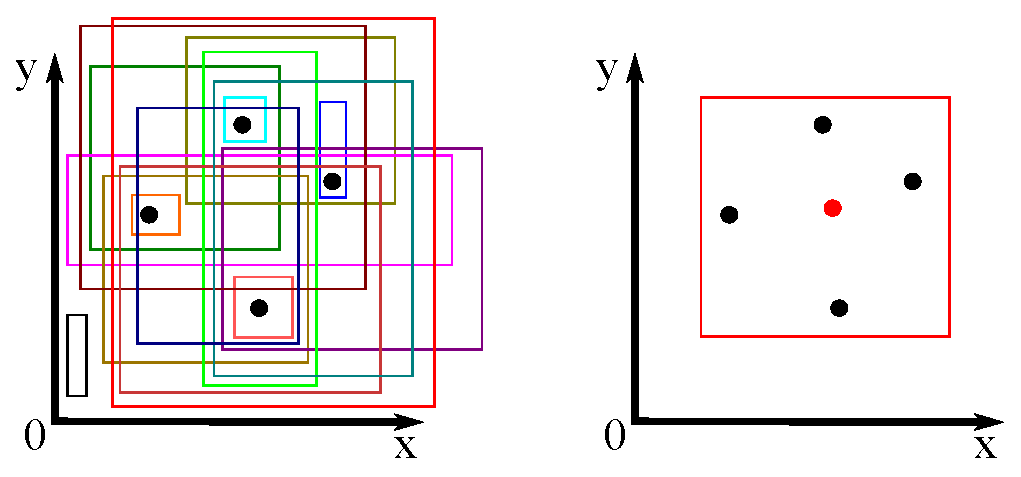
\includegraphics[width=.5\textwidth,keepaspectratio]{rectangles}
  \caption{Example of range space and VC-dimension. The space of points is the
  plane $\mathbb{R}^2$ and the set of ranges is the set of all
  \emph{axis-aligned rectangles}. The figure on the left shows graphically that
  it is possible to shatter a set of four points using 16 rectangles. On the
  right instead, one can see that it is impossible to shatter five points, as,
  for any choice of the five points, there will always be one (the red point in
  the figure) that is internal to the convex hull of the other four, so it would
  be impossible to find an axis-aligned rectangle containing the four points
  but not the internal one. Hence $\VC((X,R))=4$.}
  \label{fig:rectangles}
\end{figure}
%\begin{lemma}\label{lem:matousek}
%  The VC-Dimension of the range space $(\mathbb{R}^d, X)$, where $X$ is the set
%  of all half-spaces in $\mathbb{R}^d$ equals $d+1$.
%\end{lemma}

The main application of VC-dimension in statistics and learning theory is its
relation to the size of the sample needed to approximate learning the ranges, in
the following sense.

\begin{definition}\label{defn:eapprox}
  Let $(X,R)$ be a range space and let $A$
  be a finite subset of $X$. For $0<\varepsilon<1$, a subset $B\subset A$ is an
  $\varepsilon${\em-approximation} for $A$ if for all $r\in R$, we have
      \begin{equation}\label{eq:defeapprox}
	\left|\frac{|A\cap r|}{|A|}-\frac{|B\cap r|}{|B|}\right| \leq
	\varepsilon.
      \end{equation}
\end{definition}

%A similar definition offers relative guarantees.
%\begin{definition}\label{defn:releapprox}
%  Let $(X,R)$ be a range space and let $A$
%  be a finite subset of $X$. For $0<p,\varepsilon<1$, a subset $B\subset A$ is a
%  \emph{relative} $(p,\varepsilon)$\emph{-approximation} for $A$ if for any
%  range $r\in R$ such that $|A\cap r|/|A|\geq p$ we have 
%  \[ \left|\frac{|A\cap r|}{|A|}-\frac{|B\cap r|}{|B|}\right| \leq
%  \varepsilon\frac{|A\cap r|}{|A|}
%  \]
%  and for any range $r\in R$ such that $|A\cap r|/|A|< p$ we have $|B\cap
%	r|/|B| \leq (1+\varepsilon)p$.
%\end{definition}
%
An $\varepsilon$-approximation can be constructed by random sampling points of
the domain~[\citealp{HarPS11}, Thm.~2.12, see also~\citep{LiLS01}].

\begin{theorem}\label{thm:eapprox}
  There is an absolute positive constant $c$
  such that if $(X,R)$ is a range-space of VC-dimension at most $v$, $A\subset
  X$ is a finite subset and $0<\varepsilon,\delta<1$, then a
  random subset $B\subset A$ of cardinality $m$, where
  \begin{equation}\label{eq:eapprox}
    m\ge\min\left\{|A|,\frac{c}{\varepsilon^2}\left(v+\log\frac{1}{\delta}\right)\right\},
  \end{equation}
  is an $\varepsilon$-approximation for $A$ with probability at least $1-\delta$.
\end{theorem}

Note that throughout the work we assume the sample to be drawn \emph{with}
replacement if $m<|A|$, otherwise the sample is exactly the set $A$. The
constant $c$ is absolute and does not depend on the range space or on
any other parameter. \citet{LofflerP09} %showed 
estimated experimentally that the absolute constant $c$ is at most $0.5$. Up to
a constant, the bound presented in Thm.~\ref{thm:eapprox} is tight~\citep[Thm.~5]{LiLS01}. 

It is also interesting to note that an $\varepsilon$-approximation of size
$O(v\varepsilon^{-2}(\log v-\log\varepsilon))$ can be built
\emph{deterministically} in time
$O(v^{3v}(\varepsilon^{-2}(\log v-\log\varepsilon))^v|X|)$~\citep{Chazelle00}.


\subsection{VC-Dimension and SQL Queries}\label{sec:vcdimquer}
\citet{RiondatoACZU11} defined a range space for SQL queries and computed a
bound to its VC-Dimension. We recall here some of their results that we will use
throughout the paper.

Let $Q$ be a collection of (non-group-by, non-aggregate) queries. We define a
range space $S_Q=(X,\mathcal{R})$ associated to $Q$ as follows. The domain $X$
is the \emph{Cartesian product} of the tables involved in queries of $Q$. For
each query $q\in Q$, let $R_q$ be the subset of $X$ in the output of $q$. The
set $\mathcal{R}$ is the collection of all the ranges $R_q$ for each $q\in Q$.
In the rest of the paper we will often identify a query $q$ with its range $R_q$
(i.e., with its output) and the set of range $\mathcal{R}$ with the class of
queries $Q$. When the ranges represent all the possible outputs of queries in a class $Q$
applied to database tables $\Db$, the VC-dimension of the range space is the maximum
number of tuples such that any subset of them is the output of a query in $Q$.
The following lemmas show how to bound the VC-dimension of the
range space of different classes of queries.

\begin{lemma}[\citep{RiondatoACZU11}]\label{lem:vcdimselgen}
  Let $\Tab$ be a table with $m$ columns, let $b>0$ and let $\Sigma^{b*}_\Tab$
  be the set of selection queries on $\Tab$ whose selection predicate is a
  Boolean combination of $b$ clauses. Then, the VC-dimension of the range space
  $S_b = (\Tab, \Sigma^{b*}_\Tab)$ is at most $3((m+1)b)\log((m+1)b)$.  
\end{lemma}

\begin{lemma}[\citep{RiondatoACZU11}]\label{lem:vcdimjoinmul}
  Consider the class $Q$ of queries that can be seen as combinations of select
  and joins on $u>2$ tables $\Tab_1,\dotsc,\Tab_u$. Let $S_i=(\Tab_i,R_i)$,
  $i=1,\dotsc,u$ be the range space associated with the select queries on the $u$
  tables. Let $v_i=VC(S_i)$. Let $m$ be the maximum number of columns in a table
  $\Tab_i$. We assume $m\le \sum_i v_i$.\footnote{The assumption $m\le \sum_i
  v_i$ is reasonable for any practical case.} Let $S_Q = (\Tab_1\times\dotsb\times
  \Tab_u, R_Q)$ be the range space associated with the class $Q$. The range set
  $R_Q$ is defined as follows. Let $\rho = (r_1,\dotsc,r_u)$, $r_i\in R_i$, and
  let $\omega$ be a sequence of
  $u-1$ join conditions representing a possible way to join the $u$ tables $\Tab_i$,
  using the operators $\{>,<,\ge,\le,=,\neq\}$. We define the range 
  \[
  J^\omega_{\rho} = \{(t_1,\dotsc,t_u) ~:~ t_i\in r_i, \mbox{ s.t. }
  (t_1,\dotsc,t_u) \mbox{ satisfies } \omega\}.\]
  $R_Q$ is the set of all possible $J^\omega_{\rho}$. Then,
  \[
  VC(S_Q)\leq 4u(\sum_i VC(S_i))\log(u\sum_i VC(S_i)).
  \]
\end{lemma}

\note{We can probably remove the above two lemmas and just state the following.}
The following Theorem can be obtained by combining the above results.

\begin{theorem}\label{thm:vcdimgenqueries}
Let $b$ be a positive integer parameter. Given a set
$\Db=\{\Tab_1,\dotsc,\Tab_u\}$ of $u$ tables and a set $\mathcal{C}_i$ of
up to $m$ columns for each table $T_i$, consider the class $Q_{u,m,b}$ of all
queries on $\Db$ with up to $u-1$ join and $u$ select operations, where the
part of the selection predicate involving table $\Tab_i$ has conditions about
some of the columns from $\mathcal{C}_i$ and up to $b$ Boolean operations, then 
\[
\VC((\Db,Q_{u,m,b})) \leq 
12u^2(m+1)b\log((m+1)b)\log(3u^2(m+1)b\log((m+1)b)).\]
\end{theorem}
It is clear from this Theorem that the bound to the VC-dimension depends
only on the number of tables $u$, the number of columns $m$, and the number of
joins $b$. We can then define the function
\[
\vc(u,m,b)=12u^2(m+1)b\log((m+1)b)\log(3u^2(m+1)b\log((m+1)b)).\]

\citet{RiondatoACZU11} used Thm.~\ref{thm:eapprox} and the above bound to the
VC-dimension of the range space $S=(X,Q)$ for a collection of queries $Q$ to
compute a sample size $m$ such that a sample of size $m$ of the database can be
used to compute high-quality approximations of the selectivities of all queries
in $Q$. Formally, if we let $\sigma(q)$ be the selectivity of a query $q\in Q$
when run on the original database $\Db$ and let $\tilde\sigma(q)$ be the
selectivity of $q$ when run on the sample, \citet{RiondatoACZU11} proved that
\[
\Pr\left(\exists q\in Q \mbox{ s.t.~}
|\sigma(q)-\tilde\sigma(q)|\ge\varepsilon\right)\le\delta,
\]
for some $\varepsilon$ and $\delta$ in $(0,1)$.

\todo{Say something about how to create the sample.}

In this present work, we leverage on this result to compute good approximations
of the values of aggregate queries using a sample.

\subsection{Estimating the Selectivity of \texttt{GROUP BY} Queries}\label{sec:groupby}
To warm up, we show how to use the results introduced above to compute the
selectivity of group-by queries.

Let $\Db={\Tab_1,\dots,\Tab_u}$, and $\mathcal{C_i}$ ($1\le i \le u$), $m$, $b$,
and $Q_{u,m,b}$ be as in Thm.~\ref{thm:vcdimgenqueries}. For a positive integer
$k$, let $Q^k_{u,m,b}$ be the class of group-by queries $q(q^*,\mathcal{G})$
where $q^*\in Q_{u,m,b}$ and $\mathcal{G}=\{G_1,\dots,G_\ell\}$ is a subset of
the columns in the tables of $\Db$, under the condition that no more than $k$
columns per table are in $\mathcal{G}$. We use the equivalence from
Fact~\ref{fact:groupbyequiv} to show how to compute an approximation of the
sizes of the groups in the output of a group-by query. 

Given $\mathcal{G}$, for any query $q\in Q^k_{u,m,b}$, let $E_{q,\mathcal{G}}$
be the set of queries with selection/join predicate as
in~\eqref{eq:groupbyequiv}. It is easy to see that all $q'\in E_{q,\mathcal{G}}$
are members of the class $Q_{u,p,b+2k}$, where $p=\max\{|C_i\cap\mathcal{G}|
~:~ 1\le i\le u\}$ ($p\le m+k$. The class $Q_{u,p,b+2k}$ contains also other
queries that are not members of any $E_q$). From Thm.~\ref{thm:vcdimgenqueries},
we have that $\VC((\Db,Q_{u,p,b+2k}))\le\vc(u,p,b+2k)$.

Hence, if we build an $\varepsilon$-approximation $\Sam$ for the range space
$(\Db,Q_{u,p,b+2k})$ (for example using Theorem~\ref{thm:eapprox}) and execute
queries from $Q^k_{u,m,b}$ on $\Sam$, then the selectivities on $\Sam$ of queries
from $E_q$ will be within $\varepsilon$ from their real selectivities. Thanks to
the equivalence from Fact~\ref{fact:groupbyequiv}, this means that we can
estimate the sizes of the groups in the output of a query $q\in Q^k_{u,m,b}$ by
looking at the sizes of the groups in the output of $q$ when run on $\Sam$.

\note{I wonder whether the above should be more formal.}

Note that our guarantees do not extend to the number of groups, i.e., we cannot
guarantee that the number of groups in the output of the query when run on the
sample is within $\varepsilon$ from the number of groups in the output of the
query when run on the large database.

\section{Approximately Answering Aggregate Queries}\label{sec:aggreg}
The focus of this work is computing approximate answers to aggregate database
queries by running them on a random sample of the original database. In this
section we first describe our method to compute the \emph{point estimation}
(i.e., the estimation of the value of the query) and then show how to derive
deterministic confidence intervals for our estimations by solving convex
optimization problems.

\subsection{Point Estimation}\label{sec:pointest}
Given a database $\Db$, let $q=(q^*,f)$ be an aggregate query with
$f:\domain{C_f}\times\mathbb{N}_0\to\mathbb{R}$ for some column $C_f$ of some
table of $\Db$ (we used Fact~\ref{fact:aggregquery} to define $f$). Let $S$ be the
set of pairs $(v,c_v)$ where $v\in \domain{C_f}$ and $c_v$ is the number of times
that $v$ appears in the column $C_f$ in the output of $q^*$ when $q^*$ is run on
$\Db$.

We approximate $f(S)$, i.e., the output of $q$, with $f(\tilde{S})$ where
$\tilde{S}$ is a collection of pairs $(v,\tilde{c}_v)$ such that there is a pair
$(v,c_v)\in S$ and $c_v-\gamma_v \le\tilde{c}_v\le c+\gamma_v$ where $0\le
\gamma_v \le \gamma$, for some fixed parameter $\gamma$. In particular,
$\tilde{c}_v$ is a function of \emph{1.} the number of times that $v$ appears in the
column $C_f$ in the output of $q^*$ when $q^*$ is run on a sample, and \emph{2.}
the size of the sample.

Let $Q_{u,m,b}$ be as in Thm.~\ref{thm:vcdimgenqueries}, and let
$\mathcal{A}=Q_{u,m,b}\times\mathcal{F}$ \itodo{$\leftarrow$ Is this
the right expression?} be a class of aggregate queries $(q^*,f)$
where $q^*\in Q_{u,m,b}$ and $f\in\mathcal{F}$, for some family $\mathcal{F}$ of
functions such that each $f\in\mathcal{F}$ goes from
$\domain{\Tab.C}\times\mathbb{Z}^+$ to $\mathbb{R}$, where $\Tab.C$ is a column
in some table $\Tab$ of $\Db$. For any query $q^*\in Q_{u,m,b}$, let
$\mathcal{C}_{q^*}$ be its selection/join predicate.
We can see the output of any $q^*\in Q_{u,m,b}$ as the union of the
outputs of the queries whose selection/join predicate is $\mathcal{C}_{q^*}$
\texttt{AND}'ed with a condition on the column $C_f$, i.e., whose selection/join
predicate is in the form
\begin{equation}\label{eq:aggregselpred}
  \mathcal{C}_{q^*} \AND C_f=v;
\end{equation}
where $v\in\domain{C_f}$. Formally, let $q^*_v$ be a query with selection
predicate as in~\eqref{eq:aggregselpred}, for $v\in\domain{C_f}$, and let
$B_{q^*,f}=\{q^*_v ~:~ v\in\domain{C_f}\}$. Then, the output of $q^*$ is the union of the
outputs of all queries in $B_{q^*,f}$.

Let now $\mathsf{A}(Q_{u,m,b},\mathcal{F})$ be the union of all $B_{q^*,f}$, for
all $q^*\in Q_{u,m,b}$ and $f\in\mathcal{F}$. Consider the class
$\bar{Q}=Q_{u,m,b}\cup A(Q_{u,m,b},\mathcal{F})$. The range space $(\Db,\bar{Q})$ has
VC-dimension at most $\vc(u,m+1,b+1)$ because $\tilde{Q}$ is a subset of the
class $Q_{u,m+1,b+1}$. We can then build an $\varepsilon$-approximation $\Sam$ for
the range space $(\Db,\bar{Q})$ and the selectivity $\tilde\sigma(Q)$ of each query
$q\in\bar{Q}$ when run on $\Sam$ will be within $\varepsilon$ from its
selectivity $\sigma(q)$ when run on $\Db$. If we fix
$\varepsilon,\delta\in(0,1)$ and use Thm.~\ref{thm:eapprox} to
compute the sample $\Sam$, we have
\[
\Pr(\exists q\in\bar{Q} \mbox{ s.t. }
|\tilde\sigma(q)-\sigma(q)|\ge\varepsilon)\le\delta\enspace.
\]

Let $\eta$ be the ratio between the size of $\Db$ and the size
of $\Sam$ \itodo{Explain better what it means.}. Given an aggregate query $q\in\mathcal{A}$, we will approximate
$f(S)$ with $f(\tilde{S})$, where the members of $\tilde{S}$ are the pairs
$(v,\sigma_v\cdot\eta)$ with $\sigma_v$ being the selectivity on $\Sam$ of the
query from $A(Q_{u,m,b},\mathcal{F})$ corresponding to $(q^*,f)$ and $v$, for
all $v\in D(C)$. To compute this we do not need to run all such queries on $\Sam$ and
it suffices to run $q$ on $\Sam$. 
Note that we are not yet using the relevant properties of
$\varepsilon$-approximation (Def.~\ref{defn:eapprox}), but the advantages of
building such an $\Sam$ will be evident after the following discussion.

\note{It may look like the above discussion does not need to be that convoluted, and we
may just say that we run the query on the sample. The problem is that the result
of the query on the sample may have to be ``scaled up'' to the entire database.
Think about sum.}
\todo{Make example with sum or average?}

\paragraph{Properties of the estimation.} When using a sample to compute an
estimation for a quantity, it is highly desirable that the estimation has some
properties that make it more informative about the real value of the quantity.
One of the most desirable properties is the \emph{absence of bias}.
\todo{Describe how, in order to achieve this, one may neet/want to compute a slightly
different function for the aggregate, rather than the original. E.g.~for
variance and stddev.}
Another relevant property for the estimation is \emph{consistency}.
\todo{Same as above.}

\subsection{Deterministic confidence intervals}\label{sec:confint}
Single point estimations for a parameter $\theta$ of interes, although useful on their own, become much more
informative when accompanied with \emph{confidence intervals}. These are
intervals of the domain of $\theta$ and give information about
the accuracy of the estimation (which falls within the interval) and the
location of the real value of $\theta$. Usually,
confidence bounds are \emph{probabilistic}, in the following sense. Given a
quantity $\theta$ to be estimated, a $1-\alpha$ confidence interval $I$ is an
interval of the domain of $\theta$ such that $I$ contains $\theta$ with
probability $1-\alpha$. The probability $1-\alpha$ should be interpreted in a
frequentist framework. It represents the fraction of times that the interval
(computed according to a fix procedure) contains the real value of quantity
$\theta$, over an infinite number of repetitions of the procedure to compute the
interval. In our settings and given our goals
\itodo{which we never formally specified\ldots}, deriving probabilistic confidence bounds
is not a viable option: \todo{Here we should explain that we cannot use these
because we would have to apply a union bound over a very high number of queries,
defeating the purpose.}. Our approach instead guarantees that, if the sample
$\Sam$ is an $\varepsilon$-approximation for the range space $(\Db,Q)$ (where $Q$ is the
class of queries that one may want to run), then the confidence interval we
compute contains the real value of the query, for all aggregate queries built in
$Q$. Another advantage of our method compared to probabilistic confidence intervals
is that deriving a procedure to compute the latter is highly-specific on the
aggregate function to be estimated (e.g., average rather than standard
deviation), while our method is valid for \emph{any} aggregate function. \citet{Haas96}
developed deterministic confidence intervals for aggregate queries, but our
method computes intervals that are \emph{uniformly more powerful} than those
of~\cite{Haas96} thanks to the fact that we can leverage the properties of
$\varepsilon$-approximations.

\todo{\citep{Haas96} has some tricks that may help us getting better
estimations. Check those.}

\paragraph{The method.} Our method for computing deterministic confidence
intervals exploits the properties of the $\varepsilon$-approximation. 
In particular, we use the fact that the selectivity on $\Sam$ of all the queries in an
appropriately defined class of queries, is close (within $\varepsilon$) from
their real selectivity on $\Db$.

Let $\mathcal{A}$ \ldots \itodo{Add the others} be as in
Sect.~\ref{sec:pointest}.

Given and aggregate query $q=(q^*,f)\in$\itodo{In what?}, let $V_{q^*}(C_f)$ be
the set of values from $\domain{C_f}$ that appear in the column $C_f$ in the
output of $q^*$ when run on $\Db$. For now, assume that we know $V_{q^*}(C_f)$.
We will remove this assumption later. Consider the set
$B_{q^*,f}=\{q^*_v ~:~ v\in V_{q^*}(C_f)\}$. We want to find the sets
$E^-=\{\varepsilon^-_v ~:~ v\in V_{q^*}(C_f)\}$, $E^+\{\varepsilon^+_v ~:~ v\in
V_{q^*}(C_f)\}$ %$|\varepsilon^-_v|\le\varepsilon$, $|\varepsilon^+_v|\le\varepsilon$,
%$\left|\displaystyle\sum_{v\in V_{q^*}(C_f)}\varepsilon^-_v\right|\le\varepsilon$,
%$\left|\displaystyle\sum_{v\in V_{q^*}(C_f)}\varepsilon^+_v\right|\le\varepsilon$ and
such that the sets $\tilde{S}^-$ and $\tilde{S}^+$, whose members are
respectively the pairs
$(v,(\tilde\sigma(q^*_v)+\varepsilon^-_v)\cdot\eta)$ and
$(v,(\tilde\sigma(q^*_v)+\varepsilon^+_v)\cdot\eta)$ for all $v\in
V_{q^*}(C_f)$, are such that $f(\tilde{S}^-)$ minimizes and $f(\tilde{S}^+)$
maximizes $f(\cdot)$ among all possible choices of the sets $E^-$ and $E^+$
which satisfy some constraints explained in the following which are derived from
the fact that $\Sam$ is a $\varepsilon$-approximation.


Since we assume we can build a total order relationship on $\domain{C_f}$, let
$v_1,\dotsc,v_\ell$ be a labelling of the values in $V_{q^*}(C_f)$ in increasing
sorted order. Let $q=(q^*,f)$, and let $\mathcal{C}$ be the selection/join
predicate of $q^*$. Let $a,b$ be two values in $V_{q^*}(C_f)$. W.l.o.g.~assume
$a\le b$. Consider the query $q^*_{a,b}$ whose selection predicate is
\[
\mathcal{C} \AND C_f < a \AND C_f < b
\]
\todo{Is that $\le$ ?}
Given that $\Sam$ is a $\varepsilon$-approximation for $(\Db,Q)$ \itodo{Fix
$Q$}, we have that the selectivity $\tilde\sigma(q_{a,b})$ of $q_{a,b}$ when run on $\Sam$ is within
$\varepsilon$ from its selectivity $\sigma(q_{a,b})$ on $\Db$. More precisely,
if we let $c_{a,b}$ be the cardinality of $q_{a,b}$ on $\Db$ and $\tilde c_{a,b}$ the cardinality of
$q_{a,b}$ on $\Sam$, we have that
\[
\max\{\tilde c_{a,b},(\tilde\sigma(q_{a,b})-\varepsilon)\eta\} \le c_{a,b}\le
\min\{1, (\tilde\sigma(q_{a,b})-\varepsilon)\eta\}\enspace.\]

It should be evident that $\tilde c_{a,b}=\sum_{i=a}^b \tilde c_{i,i}$, and analogously for
$c_{a,b}$, $\sigma(q_{a,b})$, and $\tilde\sigma(q_{a,b})$. This implies that the
difference between \itodo{complete.}

The optimization problem to solve to compute the sets $E^-$ and $E^+$ is then
the following (for $E^-$, and analogously for $E^+$):
\begin{itemize}
  \item{\bf Constants:} $0\le\varepsilon\le 1$,$0\le \tilde\sigma_v\le 1, \forall v\in
    V_{q^*}(C.f)$.
  \item{\bf Variables:} $\varepsilon^-_v$ 
  \item{\bf Goal} minimize the function $f(\tilde{S}^-)$.
  \item{\bf Constraints:} 
    \begin{itemize}
      \item $\max\{0, \} \le \sum_{\ell=i}^j \sigma $.
      \item $|\varepsilon^-_v|\le\varepsilon,\forall v\in V_{q^*}(C_f)$.
      \item $\left|\displaystyle\sum_{v\in V_{q^*}(C_f)}\varepsilon^-_v\right|\le\varepsilon$.

    \end{itemize}
\end{itemize}
The properties of the $\varepsilon$-approximation are used in the constraints.
For all $v\in V_{q^*}(C_f)$, the selectivity $\sigma_v$ is within $\varepsilon$ from the
real selectivity of the query with selection/join predicate as
in~\eqref{eq:aggregselpred}, and this fact is reflected in the first constraint.
The same is true for the query $q^*$ and given that its selectivity is the sum
of the $\sigma_v$, then the absolute of the sum of the possible errors for each
of the $\sigma_v$ must be bounded by $\varepsilon$, as in the second constraint.

\begin{lemma}\label{lem:confbounds}
  For any function $f$, let $S$, $\tilde{S}^+$, and $\tilde{S}^-$ be defined as
  above. Then, $f(\tilde{S}^-)\le f(S)\le f(\tilde{S}^+)$.
\end{lemma}
\begin{proof}
  It follows from the properties of the $\varepsilon$-approximation that $S$ is
  one of the sets whose elements satisfy the constraints in the optimization
  problems. Hence, $f(S)$ is considered as a possible solution to each
  optimization problems, and the thesis follows.
\end{proof}

Until now, we assume to have perfect knowledge of $V_{q*}(C_f)$, the set of
values appearing in the column $C_f$ in the output of $q^*$ when the query is
run on $\Db$. When we run $q^*$ on a
sample (as we do to approximate the aggregate query), the output of $q^*$ may
only contain a subset $\tilde{V}_{q^*}$ of the values and if we only considered
the values in $\tilde{V}_{q*}$, the obtained confidence bounds may not contain the
real output. We therefore have to drop the assumption of knowing $V_{q^*}(C_f)$
and assume instead to know two values $m$ and $M$, with $m\le M$ such that $m$
is a lower bound to the values in $V_{q^*}(C_f)$ and $M$ is an upper bound to
the values in $V_q$. We have $V_q\subseteq[m,M]$. The values $m$ and $M$ can be
derived either from the selection predicate of $q^*$, if it involves the column
$C_f$, or are usually available, for each column, in the set of statistics
stored by the DMBS for query optimization\inote{Hass calls this the ``system
catalog'', I don't know if that is correct.}
Consider the optimization problem defined on $[m,M]$.
We have

\begin{lemma}\label{lem:equivoptprobs}
  Every solution to the optimization problem on $V_q$ is a solution to the
  optimization problem on $[m,M]$.
\end{lemma}
\begin{proof}
  By setting the variables in $[m,M]\setminus V_q$ to $0$.
\end{proof}

\begin{corollary}
  The solution to the maximization problem on $[m,M]$ is greater or equal to the
  solution to the maximization problem on $V_q$. Analogously for the
  minimization problems.
\end{corollary}


In what follows we derive analytical bounds to the confidence bounds for some
widely utilized functions. The formulas we obtain are a pessimization of the
confidence bounds found by solving the optimization problem, in the sense that
the confidence intervals obtained by using the formulas will be larger than the
one suggested by the optimization problem. The bound we derive for
$\texttt{SUM}$ is of particular interest because we will use it to derive the
other bounds.

%\paragraph{Confidence bounds for \texttt{SUM}.}
%Consider the optimization problem when the function $f$ is $\texttt{SUM}$, i.e., the output is
%the sum of the values on a given column $C$ in the tuples satisfying the selection
%predicate. Let $V_q$ be the set of values in $C$ in the output of the query $q$. The
%function to be optimized is then $\sum_{v\in V_q}(\sigma_v+\varepsilon_v)|\Db|v$,
%under the constraints $|\varepsilon_v|\le\varepsilon$ and $\sum_{v\in
%V}\varepsilon_v\le \varepsilon$. Note that we can just optimize the function
%$\sum_{v\in V_q}\varepsilon_v|\Db|v$. To express the optimization problem in standard
%form, we change the variables, substituting $\varepsilon_v$ with
%$\varepsilon^*_v=\varepsilon_v-\varepsilon$. The function to be optimized
%becomes $\sum_{v\in V_q}\varepsilon^*_v|\Db|v$, under the constraints
%$\varepsilon^*_v\le 2\varepsilon$ and $\sum_{v\in V}\varepsilon^*_v\le
%(|V|+1)\varepsilon$. 

%The optimization problem must be solved on $V_q$, but when we run $q$ on a
%sample, the output of the $q$ may only contain a subset $\tilde{V}_q$ of the
%values and if we only considered the values in $\tilde{V}_q$, the obtained
%confidence bounds may not contain the real output. Let then $m$ be a lower bound
%to the values in $V_q$ and let $M$ be an upper bound to the values in $V_q$. We
%have $V_q\subseteq[m,M]$. Consider the optimization problem defined on $[m,M]$.
%We have
%
%\begin{lemma}\label{lem:equivoptprobs}
%  Every solution to the optimization problem on $V_q$ is a solution to the
%  optimization problem on $[m,M]$.
%\end{lemma}
%\begin{proof}
%  By setting the variables in $[m,M]\setminus V_q$ to $0$.
%\end{proof}
%
%\begin{corollary}
%  The solution to the maximization problem on $[m,M]$ is greater or equal to the
%  solution to the maximization problem on $V_q$. Analogously for the
%  minimization problems.
%\end{corollary}

%Consider now the solution obtained as follows. For
%$v\in[m,m+\lceil\frac{M-m+1}{2}\rceil-2 ]$ set
%$\varepsilon^*_v=0$ and for $v\in [m+\lceil\frac{M-m+1}{2}-1\rceil,M]$ set
%$\varepsilon^*_v=2\varepsilon$. Then the corresponding value of the function to
%be optimized is a maximum. It is easy to see that the given setting of values
%corresponds to an extreme point of the convex polytope on which the problem is
%defined and that any movement from that point would result either on a
%constraint violation or on a decrement of the function to be optimized.
%
%Similarly, for the minimization problem, we set $\varepsilon^*_v=2\varepsilon$
%for $v\in[m,m+\lceil\frac{M-m+1}{2}\rceil-2]$ and $\varepsilon^*_v=0$ for
%$v\in[m+\lceil\frac{M-m+1}{2}-1\rceil,M]$.
%
%The resulting solution gives
%$\Sigma_{m,M}=\lfloor\frac{M-m+1}{2}\rfloor(\lceil\frac{M-m+1}{2}\rceil)+\varepsilon(M-m+1)M$.
%
%From now on, given an interval $[a,b]$, we will denote with $\Sigma^+_{a,b}$ the
%solution to the maximization problem on the interval $[a,b]$, and with
%$\Sigma^-_{a,b}$ the solution to the minimization problem.

\paragraph{Confidence bounds for \texttt{AVERAGE}.}

The function to be optimized would be \[
\frac{1}{\sum_{v\in V_q}(\sigma_v+\varepsilon_v)|\Db|}\sum_{v\in
V_q}(\sigma_v+\varepsilon_v)|\Db|v.\]
This function is not linear, so instead of using it, we will use a linear
function such that the confidence interval obtained by solving the optimization
problems will be larger or equal than the one obtained by using the above.
We will actually use two different functions, depending on whether we re
maximizing or minimizing. In the first case, we use the function
$\frac{1}{(\sigma_q-\varepsilon)|\Db|}\sum_{v\in V_q}(\sigma_v+\varepsilon_v)|\Db|v$.
In the second case, the function will be
$\frac{1}{(\sigma_q+\varepsilon)|\Db|}\sum_{v\in V_q}(\sigma_v+\varepsilon_v)|\Db|v$.
It is easy to see that solving the respective optimization problems will give
solutions that are worse (in an ``interval width'' sense) than the ones
obtained using the original function. What is more, we now just need to optimize
the second term of the product in each function (i.e., the sum), which we
already did in the previous Paragraph. We then obtain the following results: 

\begin{itemize}
  \item {\bf Upper Bound:} $\frac{1}{(\sigma_q-\varepsilon)|\Db|}\Sigma^+_{m,M}$.
  \item {\bf Lower Bound:} $\frac{1}{(\sigma_q+\varepsilon)|\Db|}\Sigma^-_{m,M}$.
\end{itemize}

\paragraph{Confidence bounds for \texttt{VARIANCE}.} 
The function to be optimized is 
\[
\frac{1}{(\sigma_q+\sum_{v\in V_q}\varepsilon_v)|\Db|}\sum_{v\in
V_q}(\sigma_q+\varepsilon_v)|\Db|\left(v - \frac{1}{(\sigma_q+\sum_{w\in
V_q}\varepsilon_w)|\Db|}\sum_{w\in V_q}(\sigma_q+\varepsilon_w)|\Db|w)\right).\]

We use the following equivalence, which holds for any $n>1$ and any sequence of i.i.d. random
variables $X_i$ ($\mu$ is the average of the $X_i$'s).
\[
\frac{1}{n-1}\sum_i(X_i-\mu)^2=\frac{1}{n-1}\sum_iX_i^2-\frac{1}{n^2-n}\left(\sum_iX_i\right)^2.\]

Consider now the following pair of functions. It easy to see that they are
respectively greater or equal and smaller or equal to the original function,
point by point (i.e., for the same setting of $\varepsilon_v$).
\begin{itemize}
  \item {\bf Maximization:}
    \[\frac{1}{(\sigma_q-\varepsilon)|\Db|-1}\sum_{v\in
    V_q}(\sigma_v+\varepsilon_v)|\Db|v^2-\frac{1}{(\sigma_q-\varepsilon)^2|\Db|^2-(\sigma_q+\varepsilon)|\Db|}\left(\sum_{v\in
    V_q}(\sigma_v+\varepsilon_v)|\Db|v\right)^2.\]
  \item {\bf Minimization:} 
    \[\frac{1}{(\sigma_q+\varepsilon)|\Db|-1}\sum_{v\in
    V_q}(\sigma_v+\varepsilon_v)|\Db|v^2-\frac{1}{(\sigma_q+\varepsilon)^2|\Db|^2-(\sigma_q-\varepsilon)|\Db|}\left(\sum_{v\in
    V_q}(\sigma_v+\varepsilon_v)|\Db|v\right)^2.\]
\end{itemize}

These functions are still not linear but we could bound them if we could find
upper and lower bounds to $\sum_{v\in V_q}(\sigma_v+\varepsilon_v)|\Db|v^2$. Such
upper and lower bounds, which we denote as $\Psi^+_{m,M}$ and $\Psi^-_{m,M}$ can
be found in a way similar to the one we followed for $\Sigma^+_{m,M}$ and
$\Sigma^-_{m,M}$. 

We can then derive the following bounds to the confidence interval for VARIANCE:
\begin{itemize}
  \item{\bf Upper Bound:}
\[
\frac{1}{(\sigma_q-\varepsilon)|\Db|-1}\Psi^+_{m,M}-\frac{1}{(\sigma_q-\varepsilon)^2|\Db|^2-(\sigma_q+\varepsilon)|\Db|}\times
\Sigma^-_{a,b}.\]

  \item{\bf Lower Bound:}
\[
\frac{1}{(\sigma_q+\varepsilon)|\Db|-1}\Psi^-_{m,M}-\frac{1}{(\sigma_q+\varepsilon)^2|\Db|-(\sigma-\varepsilon)|\Db|} \Sigma^+_{a,b}.\]
\end{itemize}

\paragraph{Confidence bounds for \texttt{STDEV}.} 
\todo{Square root of the ones for
VARIANCE? It looks like it.}

\paragraph{Comparison with previous results} In this Paragraph we
compare our confidence bounds with the deterministic confidence bounds presented
by Haas~\cite{Haas97}. 
\todo{Fill.}


\paragraph{Solving the optimization problems efficiently.} The constraints are convex
functions, therefore if $f$ is a convex function, the problems are
convex optimization problems and can be solved in polynomial time.
\note{It seems to be that the functions we are interested in are actually
quadratic and the constraints define a convex polytope, so it is even better.}
\todo{What else can we say here?}


\section{Experiments}\label{sec:exper}
\todo{
\begin{itemize}
  \item Evaluation of the size estimation for group-by queries. 
  \item Evaluation of the aggregate function estimation. 
  \item Evaluation of the confidence bounds with comparison with the
    deterministic confidence bounds from~\cite{Haas97}.
\end{itemize}
}


\section{Previous Work}\label{sec:prevwork}
\todo{This needs to be revised.}
Many of the early contributions and developments in the area of Approximate
Query Processing (AQP) using sampling are presented in the survey by~\citet{Das09}. Here we focus on the contributions that are more related to
ours.

Using workload information to improve the quality of AQP was explored by many
authors~\citep{KonigW99,GantiLR00,ChaudhuriDDMN01,LazaradisM01,ChaudhuriDN07}. The
usual approach is to use this information to assign different weights to the
tuples in the database and then use weighted sampling to ensure that tuples that
are used more often have higher probability of appearing in the sample. Although
we also develop our results for classes of queries representing the workload of
the database, these classes can be completely defined by their SQL expression
and are therefore completely data-independent, with the effect of making our
results much more general and flexible.

\citet{Haas96,Haas97} developed Hoeffding-like inequalities to derive
accurate estimations of query answers and confidence bounds to them.
Simultaneous statistical inference techniques like the union
bound~\citep{Miller81} must be used in order to derive uniform guarantees over a
class of queries, which are known to be overly conservative when the number of
queries is large.  The work is nevertheless interesting because it presents a
class of deterministic confidence intervals which can be compared with the ones
we present in Sect.~\ref{sec:aggreg}.

In the work by~\citet{ChaudhuriDN07}, the solution of an
optimization problem suggests good strata into which partition the tuples,
before using stratified sampling, in order to achieve higher quality in AQP.
The obtained sample is such that the mean square error in estimating the
selectivity of queries belonging to a given workload is minimized, but there is
no quality guarantee on the maximum error. We instead solve optimization
problems to find confidence bounds to our estimate of the query answer, giving a
guarantee on the error we make.

\citet{PolJ05} use the bootstrap, a statistical tool, to derive
confidence bounds to the estimates. In its simplest form, their work requires
running the query multiple (possibly thousands) of times, but additional data
structures allows for running the query only once. The major difference from our
work is that the boostrap gives \emph{experimental} confidence bounds, while we
give an \emph{analytical} procedures and guarantees to derive the bounds.

The work of~\citet{XuJD08} also deals with developing confidence bounds
to estimates of answers to queries involving \texttt{GROUP BY} conditions. They
suggest that correlation between groups answers should be taken into account
when computing the bounds. This can be done by solving an inference problem
which can not be solved in polynomial time unless $P=NP$. The authors examine
different heuristics to circumvent this limitation. In our work we do not need
to take correlation between groups into account because the guarantees on the
group size estimates hold uniformly and independently for all groups.

\citet{RoschL09} suggest a biased sample approach to improve
the quality of estimates for small-sized groups. Their technique exploits the
standard deviation of the aggregate values in a group to compute how many tuples
from that group should be sampled. In order to do this, a fixed set of aggregate
attributes must be specified. Our approach, on the other hand, is much more
general in that we do not need this information, and aggregates can be computed
on any column.

\citet{AgarwalMPMMS13} present BlinkDB, a parallel engine for query processing
that uses stratified sampling to approximate aggregate queries. BlinkDB exploits
query workload information to select the best group of columns for the strata.
The samples are selected depending on the query and on additional constraints on
runtime and accuracy specified by the user. The system can not actually
guarantee that the estimation has the required accuracy for all queries, as no
correction for multiple queries (e.g.~the union bound) is considered when
computing sample size. On the contrary, our approach guarantees that, with
probability at least $1-\delta$, the confidence interval it compute contains the
real value for all queries.


\section{Conclusions}\label{sec:concl}
\todo{Fill.}



\bibliographystyle{plainnat}
\bibliography{approxbib,riondapubs,vcfreq,vcmine}

\end{document}

